
\documentclass[11pt]{beamer}
\usetheme{Warsaw}
\usepackage[utf8]{inputenc}
\usepackage[russian]{babel}
\usepackage[T2A]{fontenc}
\usepackage{amsmath}
\usepackage{amsfonts}
\usepackage{amssymb}
\usepackage{graphicx}
\author{Турганбаев Сатбек}
\title{Исследование метода восстановления волнового фронта }
\subtitle{по его наклонам на основе вейвлетов Хаара}
%\setbeamercovered{transparent} 
%\setbeamertemplate{navigation symbols}{} 
%\logo{} 
\institute{Московский Государственный Университет имени М.В.Ломоносова \\
Факультет вычислительной математики и кибернетики \\
Кафедра математической физики \\
\vspace{\baselineskip}
Выпускная квалификационная работа бакалавра \\
\vspace{\baselineskip}
Научный руководитель: д.т.н., профессор Разгулин А.В.} 
\date{2018} 


\setbeamertemplate{navigation symbols}{}

\begin{document}










\begin{frame}
	\thispagestyle{empty}
	\begin{rm}
	\begin{center}
		
		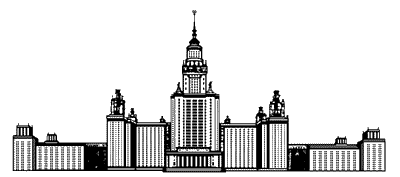
\includegraphics[width=0.2\textwidth]{msu_logo_small.png}\\
		\scriptsize \textsc { Московский государственный университет имени М.~В.~Ломоносова\\
		Факультет вычислительной математики и кибернетики\\
		Кафедра математической физики}
		
		\vspace{0.6 cm}
		
		\small{ Турганбаев Сатбек Амангельдыулы}
		
		\vspace{0.6 cm}
		
	        \large \textbf { Исследование метода восстановления волнового фронта по его наклонам на основе вейвлетов Хаара }

		\vspace{0.6 cm}
		
		\scriptsize  {ВЫПУСКНАЯ КВАЛИФИКАЦИОННАЯ РАБОТА }
	\end{center}
	
		\vfill
	
	\begin{flushright}
		\scriptsize{
		\textbf{Научный руководитель:}\\
		д.ф-м.н.\\
                Разгулин Александр Витальевич
               }
	\end{flushright}
	
	\vfill
	
	\begin{center}
		\small{Москва, 2018}
	\end{center}

	\end{rm}
\end{frame}
\begin{frame}
\frametitle{Цель работы}
\begin{itemize}

\item Реализовать вейвлет метод
\item Проверить работу метода на различных $g_1,\,g_2$
\item Реализовать вариационный метод
\item Исследовать случай восстановления по средним локальным апертурам значений наклонов

\end{itemize}

\end{frame}

\begin{frame}
\frametitle{Вейвлет метод}
\begin{center}
			$$g_1= \frac{u(x_i,y_j) - u(x_{i-1},y_j)}{h_1}$$
			$$g_2= \frac{u(x_i,y_j) - u(x_i,y_{j-1})}{h_2}$$
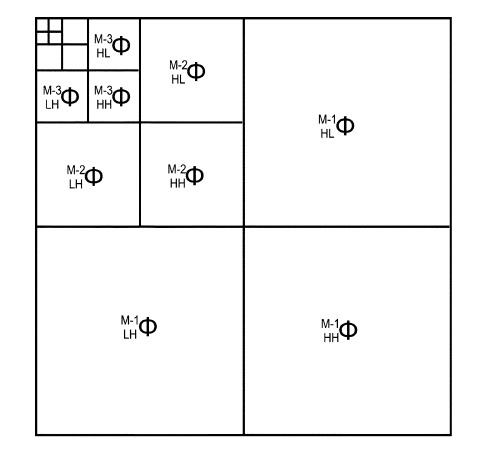
\includegraphics[width=0.5\textwidth]{hwaf_decomp.png}

\end{center}
\end{frame}



\begin{frame}
\frametitle{Первые разностные производные}
\begin{center}
$$g_1= \frac{u(x_i,y_j) - u(x_{i-1},y_j)}{h_1}$$
$$g_2= \frac{u(x_i,y_j) - u(x_i,y_{j-1})}{h_2}$$
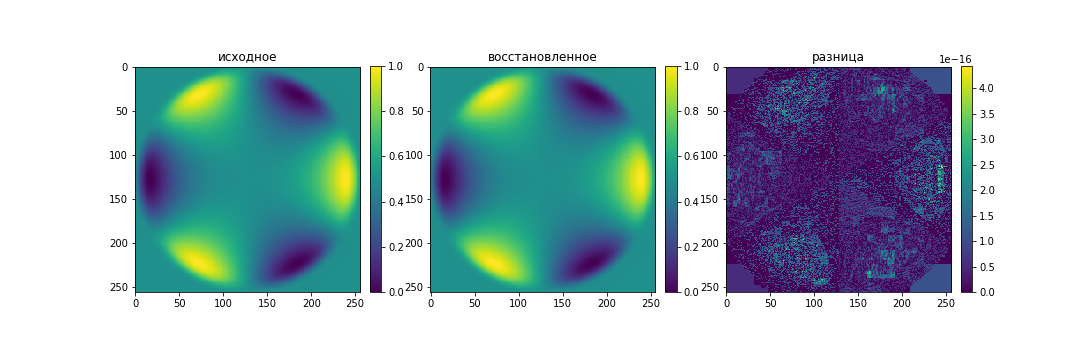
\includegraphics[width=1\textwidth]{Z_3^3.png}
\end{center}
\end{frame}

\begin{frame}
\frametitle{Точные значение производных}
$$g_1 = u_x(x_i,y_j);\; g_2 = u_y(x_i,y_j)$$
\begin{center}
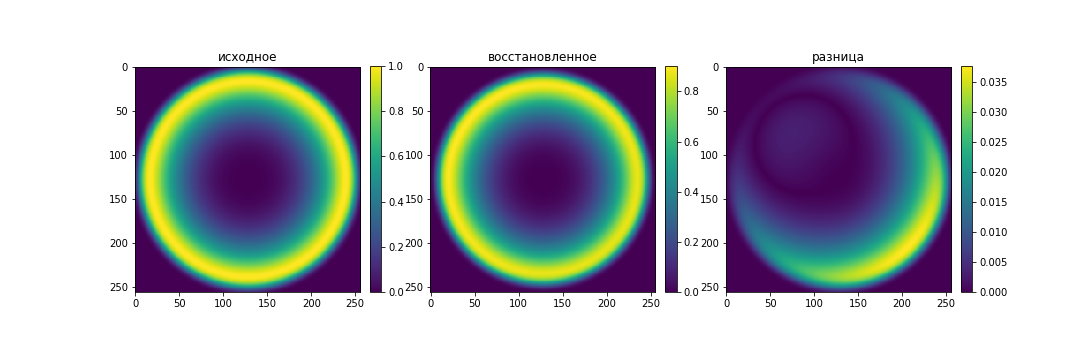
\includegraphics[width=1\textwidth]{R_3^3_variant1.png}
\end{center}
\end{frame}

\begin{frame}
\frametitle{Вариационный метод}
 $$J(u) = \int \limits_0^{2\pi} \int \limits_0^{2\pi} ((u_x - g_1)^2 + (u_y-g_2)^2 + \alpha u^2 )dxdy \rightarrow min$$
 $$(u_x, \phi_x) + (u_y,\phi_y) + \alpha(u, \phi) = (g_1, \phi_x) + (g_2, \phi_y),\;\;\forall\phi \in W_{2\pi}^{1}(\Omega)$$
 $$B_2 \Lambda_1 u + B_1 \Lambda_2 u + \alpha B_1 B_2 u + \gamma\Lambda_1\Lambda_2u = F(g_1,g_2)$$
 
$$u_{kl} = \frac{f_{kl}}{\mu_l \lambda_k + \mu_k \lambda_l + \alpha \mu_k \mu_l + \gamma \lambda_k \lambda_l}$$
\end{frame}

\begin{frame}
\frametitle{$g_1,\,g_2$}
$$g_1 = u_x(x_i,y_j);\; g_2 = u_y(x_i,y_j)$$
$$
g_1 = \frac{1}{h_1h_2} \sum \limits_{n=1}^{N_1 - 1} \sum \limits_{m=1}^{N_2 - 1} \int \limits _{\Delta_{nm}} u_\xi(\xi,\eta) d\xi d\eta\overset{\circ}{\varphi}_{nm}(x,y)
$$
$$
g_2 = \frac{1}{h_1h_2} \sum \limits_{n=1}^{N_1 - 1} \sum \limits_{m=1}^{N_2 - 1} \int \limits _{\Delta_{nm}} u_\eta(\xi,\eta) d\xi d\eta \overset{\circ}{\varphi}_{nm}(x,y)
$$

$$
\Delta_{nm} = [x_{n-1}, x_n] \cup [y_{n-1}, y_n]
$$
$$
\overset{\circ}{\varphi}_{nm}(x,y) = \begin{cases} 1, \, x \in \Delta_{nm} \\ 0, \, else\end{cases}
$$

\end{frame}

\begin{frame}
\frametitle{Частотная характеристика}
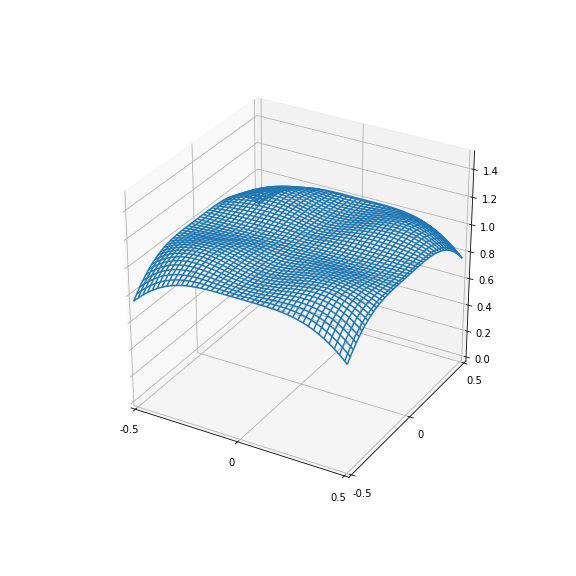
\includegraphics[width=0.8\textwidth]{3dcont.png}
\end{frame}

\begin{frame}
\frametitle{Частотная характеристика}
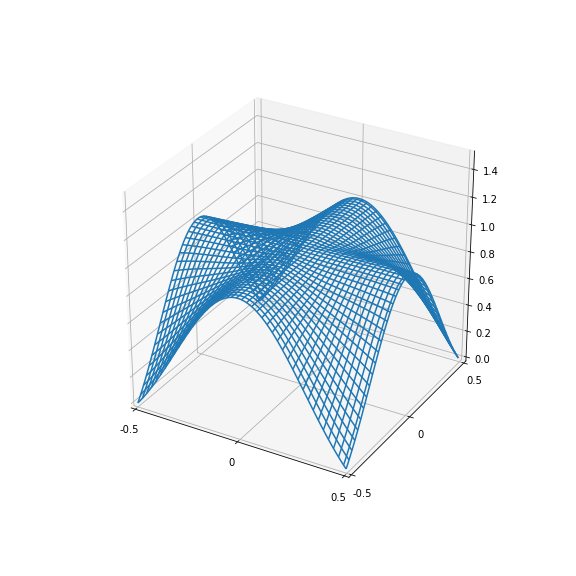
\includegraphics[width=0.8\textwidth]{3dpiece.png}
\end{frame}

\begin{frame}
\frametitle{Частотная характеристика}
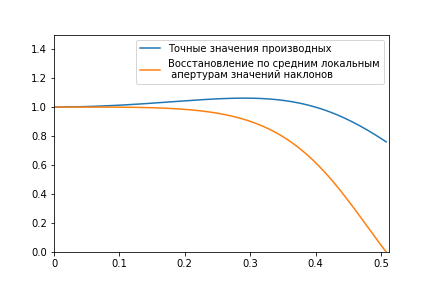
\includegraphics[width=0.8\textwidth]{2cases.png}
\end{frame}


\begin{frame}
\frametitle{Восстановление полиномов Цернике}
\begin{center}

\begin{figure}[h]
\begin{minipage}[h]{0.49\linewidth}
\center{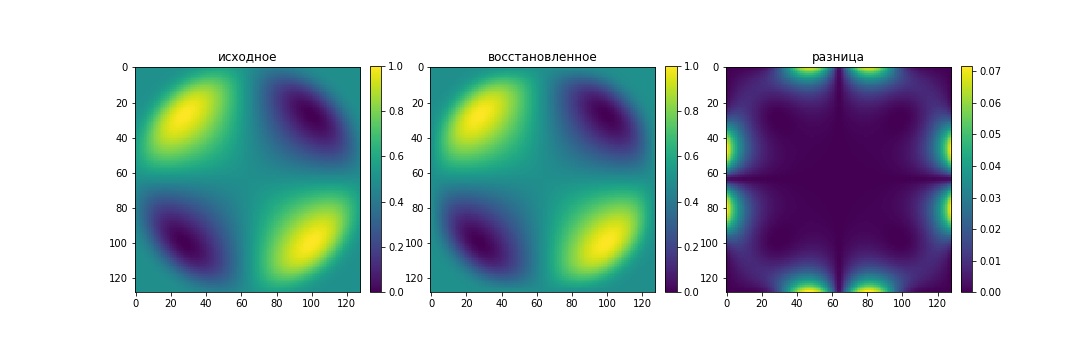
\includegraphics[width=1.5\linewidth]{z_2^-2.png} }
\end{minipage}
\vfill
\begin{minipage}[h]{0.49\linewidth}
\center{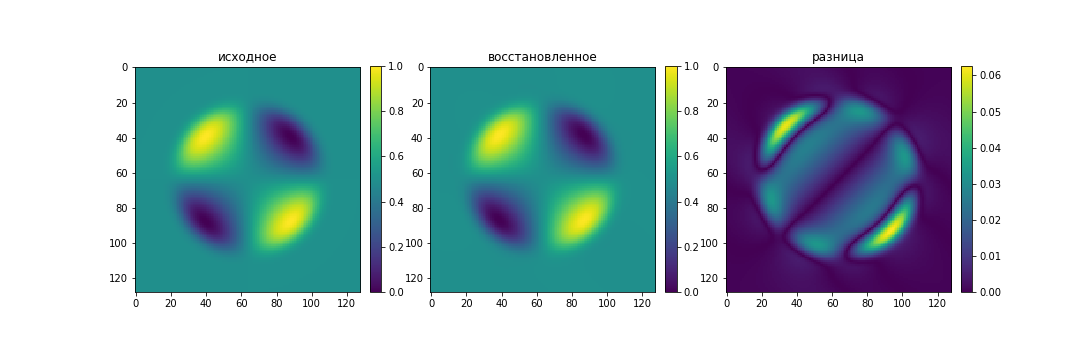
\includegraphics[width=1.5\linewidth]{z_2^-2_v2.png}}
\end{minipage}
\end{figure}

\end{center}
\end{frame}



\end{document}
